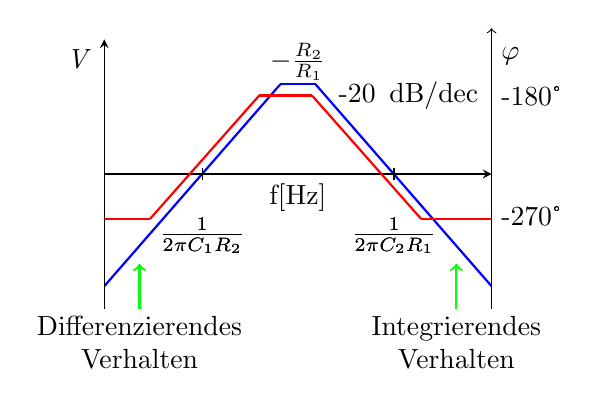
\begin{tikzpicture}[scale=1, transform shape]
    \begin{axis}[
        width=6.5cm, % Breite des Graphen
        height=5cm, % Höhe des Graphen
        xmin=0, xmax=11,
        ymin=-1.2, ymax=1.2,
        axis lines=center,
        axis on top=true,
        domain=0:10,
        clip mode=individual, % Verhindert das Abschneiden von Elementen
        xtick=\empty,
        ytick=\empty,
        ylabel style={xshift=-0.6cm},
        ylabel={\it V},
        xlabel={f[Hz]},
        xlabel style={at={(axis description cs:0.5,0.5)},anchor=north}
        ]
        \path[draw=none] (axis cs:-2, 0) rectangle (axis cs:13,1); \path[draw=none] (axis cs:-2, 0) rectangle (axis cs:13,1);


        \addplot+[mark=none, thick, blue] coordinates {(0,-1) (5,0.8)};
        \addplot+[mark=none, thick, blue] coordinates {(5,0.8) (6,0.8)};
        \addplot+[mark=none, thick, blue] coordinates {(6,0.8) (11,-1)};
        \node[anchor=north] at (axis cs:5.5,1.25) {$-\frac{R_2}{R_1}$};
        \addplot+[only marks, mark=|, black] coordinates {(2.78,0)} node[anchor=south] at (axis cs:2.78,-0.8) {$\frac{1}{2 \pi C_1 R_2}$};
        \addplot+[only marks, mark=|, black] coordinates {(8.23,0)} node[anchor=south] at (axis cs:8.23,-0.8) {$\frac{1}{2\pi C_2 R_1}$};
        \node[anchor=east] at (axis cs:10.9,0.7) {-20\, \text{dB/dec}};
        \addplot+[only marks, mark=|, black] coordinates {(2.78,0)} node[anchor=south] at (axis cs:2.78,-0.8) {$\frac{1}{2 \pi C_1 R_2}$};
        \addplot+[only marks, mark=|, black] coordinates {(8.23,0)} node[anchor=south] at (axis cs:8.23,-0.8) {$\frac{1}{2\pi C_2 R_1}$};
        \draw[->, thick, green] (axis cs:1,-1.2) -- (axis cs:1,-0.8);
        \node[align=center, black] at (axis cs:1,-1.5) {Differenzierendes\\ Verhalten};
        
        \draw[->, thick, green] (axis cs:10,-1.2) -- (axis cs:10,-0.8);
        \node[align=center, black] at (axis cs:10,-1.5) {Integrierendes\\ Verhalten};
        
    \end{axis}
    
    \begin{axis}[
        width=6.5cm, % Breite des Graphen
        height=5cm, % Höhe des Graphen
        xmin=0, xmax=11,
        ymin=0, ymax=240, 
        axis y line*=right,
        axis x line=none,
        ylabel={$\varphi$},
        ylabel style={rotate=270, anchor=west, yshift=1.5cm},
        xtick=\empty,
        ytick=\empty,
        clip mode=individual, % Verhindert das Abschneiden von Elementen
        after end axis/.code={
            \draw[->] (axis cs:11,240) -- (axis cs:11,250);
        }
        ]
        \addplot+[mark=none, thick, red] coordinates {(0,80) (1.3,80)};
        \addplot+[mark=none, thick, red] coordinates {(1.3,80) (4.4,190)};
        \addplot+[mark=none, thick, red] coordinates {(4.4,190) (5.9,190)};
        \addplot+[mark=none, thick, red] coordinates {(5.9,190) (9,80)};
        \addplot+[mark=none, thick, red] coordinates {(9,80) (11,80)};
        \node[anchor=west] at (axis cs:11,82.5) {-270°};
        \node[anchor=west] at (axis cs:11,190) {-180°};
       
    \end{axis}

    
    \end{tikzpicture}